\chapter{Superficies}%
\label{cha:superficies}
\section{Concepto}%
\label{sec:concepto_sup}
\begin{defi}
Una \underline{superficie} es un espacio localmente homeomorfo a $\mathbb{R}^{2}$. Supondremos siempre que es $T_2$ y el II Ax., lo que implica que se puede sumergir en $\mathbb{R}^{n}$ para $n$ grande.
\end{defi}
Nos interesan las superficies \underline{compactas}. Las tres primeras son cocientes:
%TODO: Imagen
\begin{center}
    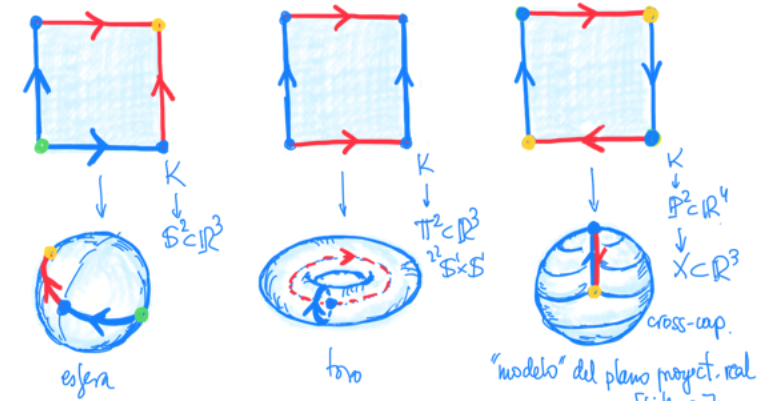
\includegraphics[scale=0.3]{images/primeras_superficies} 
\end{center}
\underline{Ejercicio}: $\mathbb{P}^{2} \xhookrightarrow{} \mathbb{R}^{4}: \left( x_0 : x_1 : x_2 \right) \mapsto \frac{\left( x_1^2 - x_2^2, x_0x_1, x_0x_2, x_1x_2 \right)}{x_0^2 + x_1^2 + x_2^2}$.

\begin{obs}
$P^2 \rightarrow \mathbb{R}^{3}$ tiene siempre identificaciones adicionales (como el cros-cap?)
\end{obs}

\section{Sumas conexas}%
\label{sec:sumas_conexas}
El método genérico para construir superficies requiere el concepto un poco más general siguiente:
\begin{defi}
Una superficie \underline{con borde} es un espacio local homeomorfo a $\{x \ge 0\} \subset \mathbb{R}^{2}$ y los puntos del borde se corresponden con $\{x = 0\}$ (es una definición consistente por la inversa? del borde)
%TODO: Imagen
\begin{center}
    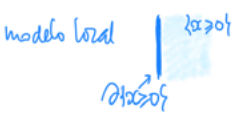
\includegraphics[scale=0.3]{images/def_con_borde} 
\end{center}
\end{defi}
\begin{obs}
Sin los puntos del borde se tiene una superficie ordinaria.
\end{obs}

\begin{ej}
\begin{enumerate}
    \item Un disco cerrado, que tiene por borde la circunferencia.
    \item Una corona circular, una banda entre rectas paralelas, un tronco de cilindro. 
    %TODO: Imagen
    \begin{center}
        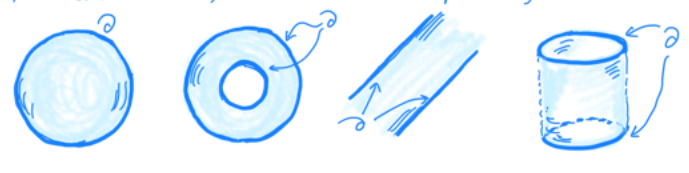
\includegraphics[scale=0.3]{images/ej_con_borde} 
    \end{center}
\end{enumerate}
\end{ej}

Con este concepto podemos ``hacer agujeros'' en superficies y, con ellos, definir:
\begin{defi}
La \underline{suma conexa} $M \# M'$ de dos superficies $M$ y $M'$ se construye haciendo un agujero en cada una y pegando las superficies agujereadas por sus bordes:
\begin{enumerate}
    \item Agujeros: $B \subset M$ y $B \subset M'$ (discos abiertos) con bordes $S = \overline{B} \setminus B$ y $S' = \overline{B'} \setminus B'$ (circunferencias).
    \item Superficies agujereadas: $M\setminus B$ y $M'\setminus B$ con los mismos bordes $S$ y $S'$.
    \item Pegando por los bordes: $M \# M' = \left( \left( M \setminus B \right) + \left( M' \setminus B' \right) \right) / \left( S \equiv S' \right)$.
    %TODO: Imagen
    \begin{center}
        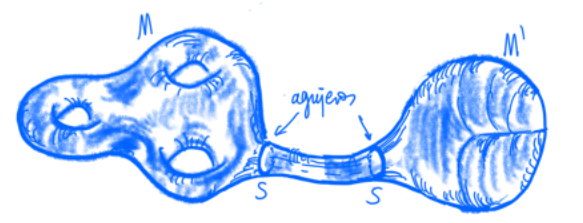
\includegraphics[scale=0.3]{images/def_suma_conexa} 
    \end{center}
\end{enumerate}
\end{defi}

\begin{prop}
La suma conexa está bien definida y no depende de los agujeros elegidos (salvo homeomorfismos).
\end{prop}
\begin{demo}
Que efectivamente es una superficie ordinaria (sin borde) es fácil si elegimos los agujeros en abiertos de las superficies homeomorfas a $\mathbb{R}^{2}$. Luego, hay que ver que si cambiamos los agujeros obtenemos el mismo resultado (salvo homeomorfismo) y esto ya requiere resultados profundos como el teorema de Jordan-Schoenflies.
\end{demo}

\begin{prop}
La suma conexa es una operación asociativa conmutativa con elemento neutro la esfera.
\end{prop}
\begin{demo}
Que $\left( M \# M' \right) \# M'' \approx M \# \left( M' \# M'' \right)$ es fácil tomando agujeros bien separados. También es obvio que $M \# M' \approx M' \# M$. Finalmente:
\[
M \# \mathbb{S}^{2} = \left( \left( M \setminus B \right) + \left( \mathbb{S}^{2} \setminus B' \right) \right) / \left( S \equiv S' \right) = \left( \left( M \setminus B \right) + B \right) / \left( S \equiv S' \right) = M
\]
pues $\mathbb{S}^{2} \setminus B'$ es un disco cerrado que restituimos a $M$.
\end{demo}

\section{Cocientes}%
\label{sec:cocientes_sum_conx}
Las sumas conexas se visualizan muy bien mediante identificaciones.
\begin{enumerate}
    \item \underline{Suma conexa de toros}: 
    %TODO: Imagen
    \begin{center}
        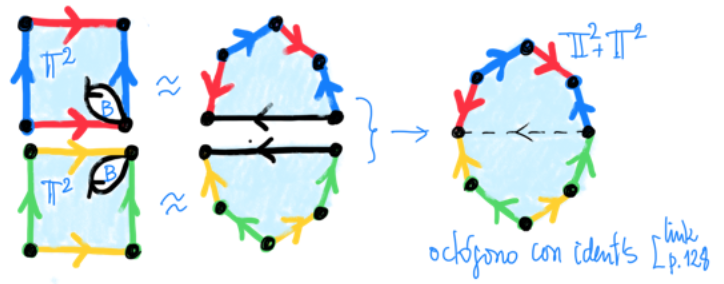
\includegraphics[scale=0.3]{images/sum_conx_toros} 
    \end{center}

    \item \underline{Suma conexa de planos proyectivos}:
    %TODO: Imagen
    \begin{center}
        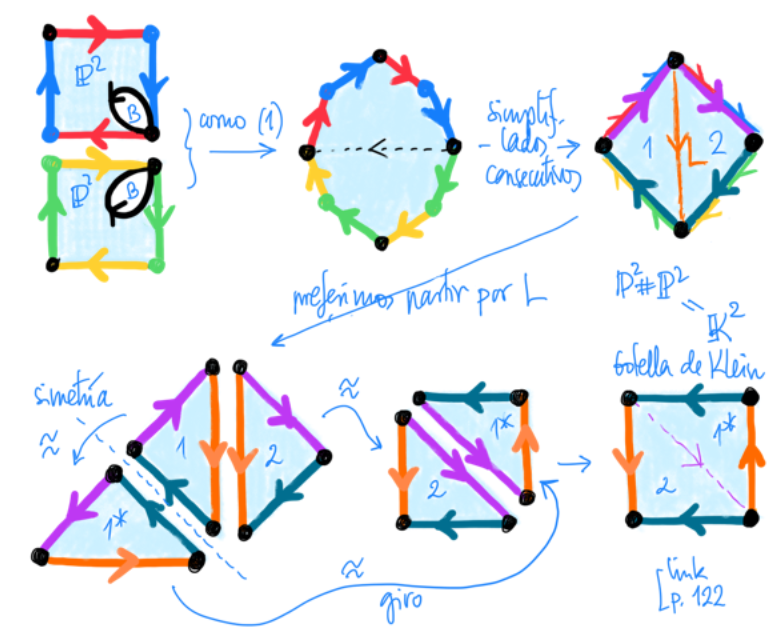
\includegraphics[scale=0.3]{images/sum_conx_planos_proy} 
    \end{center}
\end{enumerate}


\chapter{Clasificación de superficies}%
\label{cha:clasificacion_de_superficies}
\section{El teorema}%
\label{sec:el_teorema}
\begin{theo}
Toda superficie compacta es homeomorfa a una y sólo una entre:
\[
\mathbb{S}^{2};\ \Pi^2 \# \stackrel{k}{\cdots} \Pi^2, k\ge 1;\ \mathbb{P}^{2} \# \stackrel{k}{\cdots} \# \mathbb{P}^{2}, k\ge 1 
\]
\end{theo}
Las podemos dibujar:
\begin{itemize}
    \item En $\mathbb{R}^{3}$:
    %TODO: Imagen
    \begin{center}
        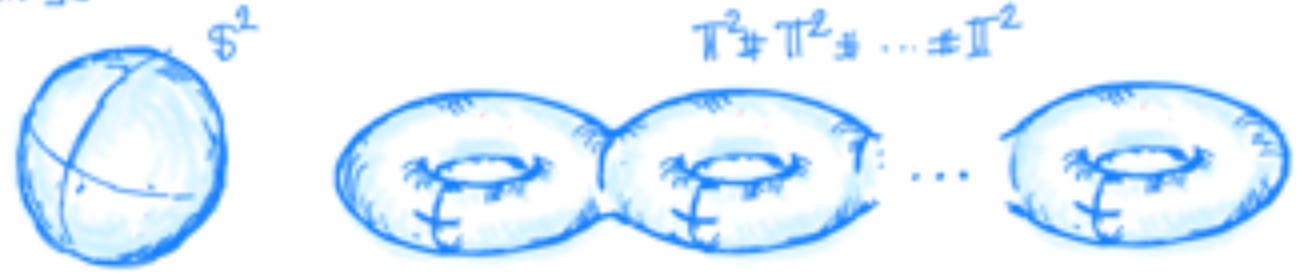
\includegraphics[scale=0.3]{images/superficies_r3} 
    \end{center}
    \item En $\mathbb{R}^{4}$ (modelo en $\mathbb{R}^{3}$):
    %TODO: Imagen
    \begin{center}
        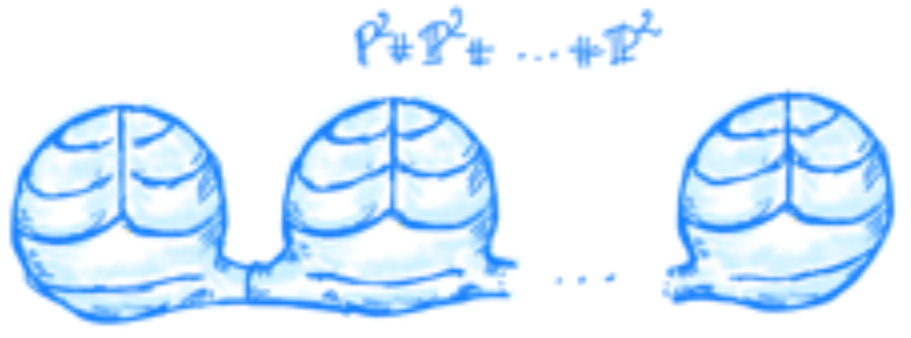
\includegraphics[scale=0.3]{images/superficies_r4} 
    \end{center}
\end{itemize}
El ``solo una'' del enunciado nos dice que estas superficies son \underline{todas distintas} (no homeomorfismo): el grupo fundamental las distingue. Ya sabemos que $\pi\left( \mathbb{S}^{2} \right) = \{1\},\ \pi\left( \Pi^2 \right) = \mathbb{Z}^2,\ \pi\left( \mathbb{P}^{2} \right) = \mathbb{Z}_2$ y los demás $H_0?$ son desiguales (aunque no sepamos calcularlos).

\section{La relación fundamental}%
\label{sec:la_relacion_fundamental}
En la lista del teorema de clasificación no hay sumas ``mixtas'': $\Pi^2 \# \mathbb{P}^{2},\ldots$, pero el mismo teorema nos dice que están en la lista. Es claro que, por las propiedades de $\#$, cualquier suma conexa de $\mathbb{S}^{2}, \Pi^2$ y $\mathbb{P}^{2}$ estará en la lista en cuanto esté $\Pi^2 \# \mathbb{P}^{2}$. En efecto:

\begin{prop}
$\mathbb{P}^{2} \# \Pi^2 = \mathbb{P}^{2} \# \mathbb{P}^{2} \# \mathbb{P}^{2}$.
\end{prop}
\begin{demo}
    ``Cut \& paste'' típico de identificaciones. Como $\mathbb{P}^{2} \# \mathbb{P}^{2} = \mathbb{K}^2$ (\ref{sec:cocientes_sum_conx}) es la botella de Klein, el homeomorfismo que partiremos? es $\mathbb{P}^{2} \# \Pi^2 = \mathbb{P}^{2} \# \mathbb{K}^2$ con:
    %TODO: Imagen
    \begin{center}
        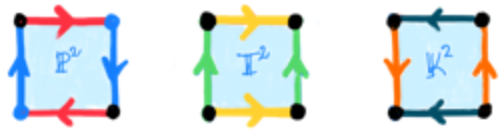
\includegraphics[scale=0.3]{images/rel_fund_1} 
    \end{center}

    \begin{enumerate}
        \item Agujeros:
        %TODO: Imagen
        \begin{center}
            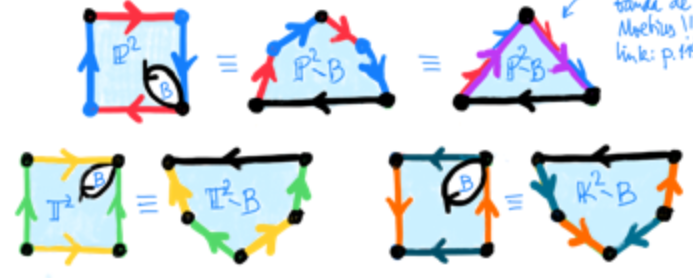
\includegraphics[scale=0.3]{images/rel_fund_agujeros} 
        \end{center}

        \item Pegados:
        %TODO: Imagen
        \begin{center}
            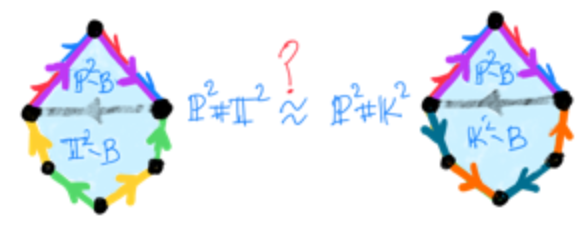
\includegraphics[scale=0.3]{images/rel_fund_pegados} 
        \end{center}

        \item \textit{Cut \& paste}:
        %TODO: Imagen
        \begin{center}
            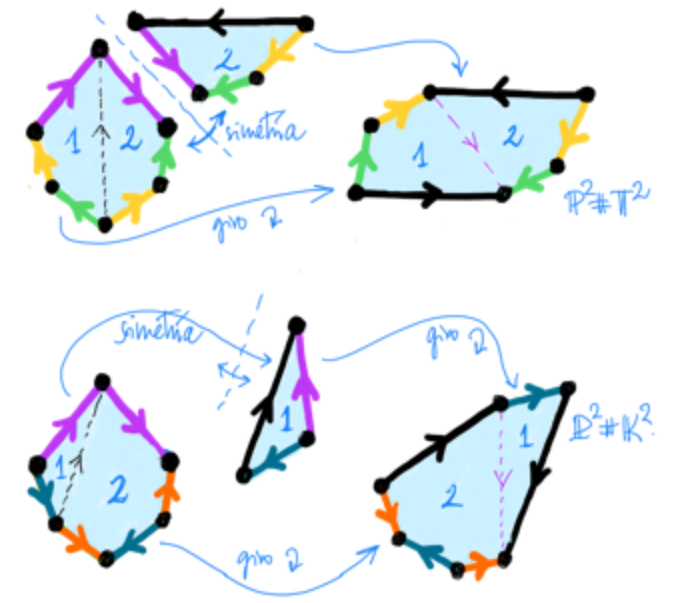
\includegraphics[scale=0.3]{images/rel_fund_c&p} 
        \end{center}
    \end{enumerate}
    Obtenemos dos representaciones nuevas de $\mathbb{P}^{2} \# \Pi^2$ y $\mathbb{P}^{2} \# \mathbb{K}^2$, con apariencias desiguales, pero topologías iguales: dos hexágonos con las mismas identificaciones de lados:
    %TODO: Imagen
    \begin{center}
        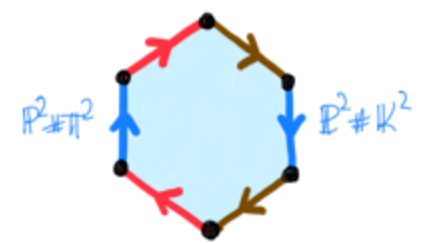
\includegraphics[scale=0.3]{images/rel_fund_hex} 
    \end{center}
    No dejarse engañar por los colores ni los sentidos de las flechas.
\end{demo}

\section{Grupos fundamentales con un agujero}%
\label{sec:grupos_fundamentales_con_un_agujero}
Aunque no podamos distinguir todas las superficies unas de otras porque no conocemos todos los grupos fundamentales, si podemos hacer algunas distinciones ``haciendo agujeros''.

\begin{prop}
Distinguimos:
\begin{enumerate}
    \item $\pi\left( \mathbb{S}^{2} \setminus \{a\} \right) = \pi\left( \mathbb{R}^{2} \right) = \{1\}$.
    \item $\pi\left( \Pi^2 \# \stackrel{k}{\cdots} \# \Pi^2 \setminus \{a\} \right) = \pi\left( dibujo^{2k}  \right) = \mathbb{Z}^{*^{2k}}$.
    \item $\pi\left( \mathbb{P}^{2} \# \stackrel{k}{\cdots} \# \mathbb{P}^{2} \setminus \{a\} \right) = \pi\left( dibujo^{k} \right) = \mathbb{Z}^{*^{k}}$.
\end{enumerate}
\end{prop}
\begin{demo}
Tenemos
%TODO: Imagen. Ni idea de como hacerlo
\begin{center}
    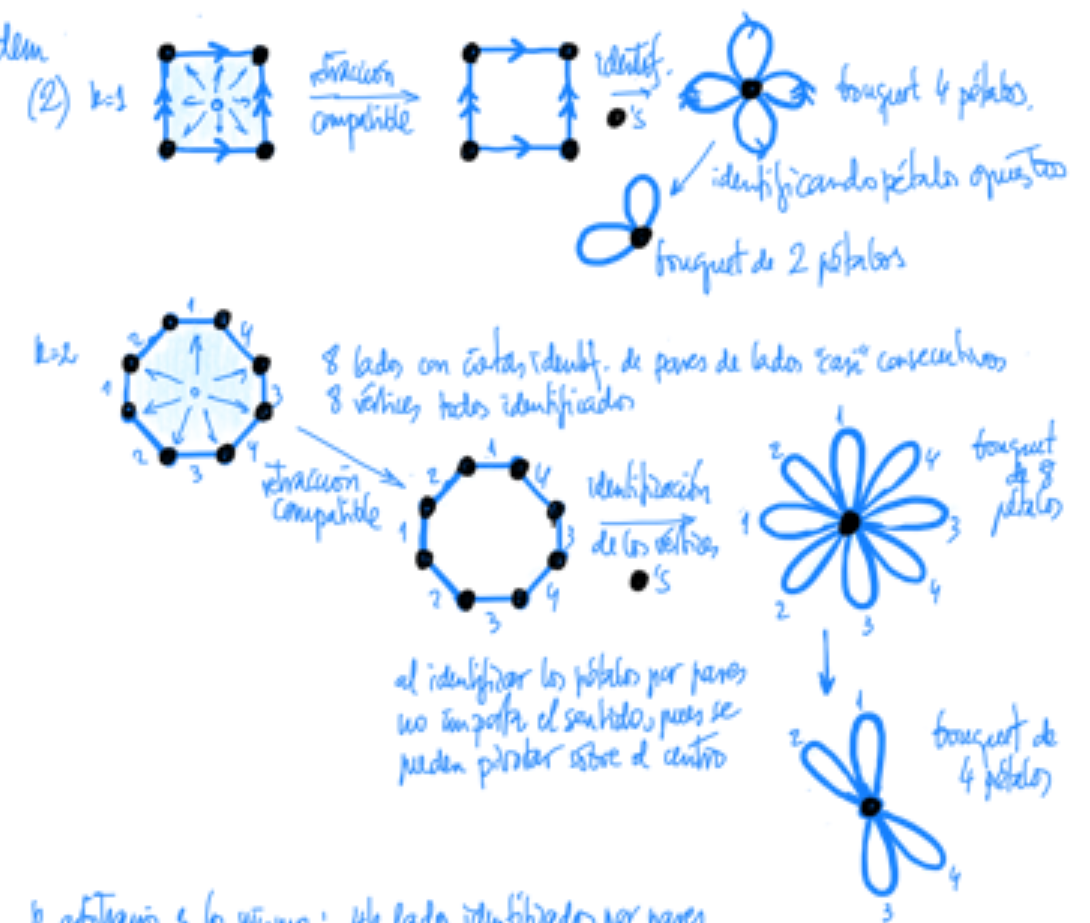
\includegraphics[scale=0.3]{images/dem_grupos_fund_agujeros} 
\end{center}
\end{demo}

Con $k$ arbitrario es lo mismo: $4k$ lados identificados por pares, $4k$ vértices todos identificados. Por retracción radical desde un punto interior (el agujero), obtenemos la poligonal con esas mismas identificaciones. Al identificar los vértices se tiene un bouquet de $4k$ pétalos y, al identificar pétalos por pares, un bouquet de $2k$ pétalos.
\begin{demo}
%TODO: Imagen
\begin{center}
    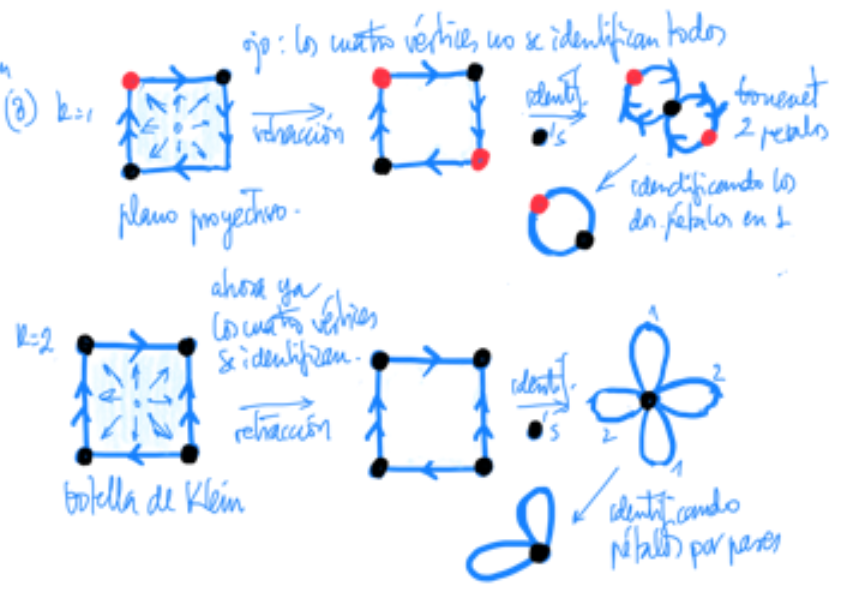
\includegraphics[scale=0.3]{images/dem_grupo_fund_agujeros_2} 
\end{center}    
$k = 3$. Por \textit{cut \& paste}, los lados, pueden? sumar un proyectivo aporta? $2$ lados identificados entre sí con tres vértices identificados todos (\ref{sec:la_relacion_fundamental}).
%TODO: Imagen
\begin{center}
    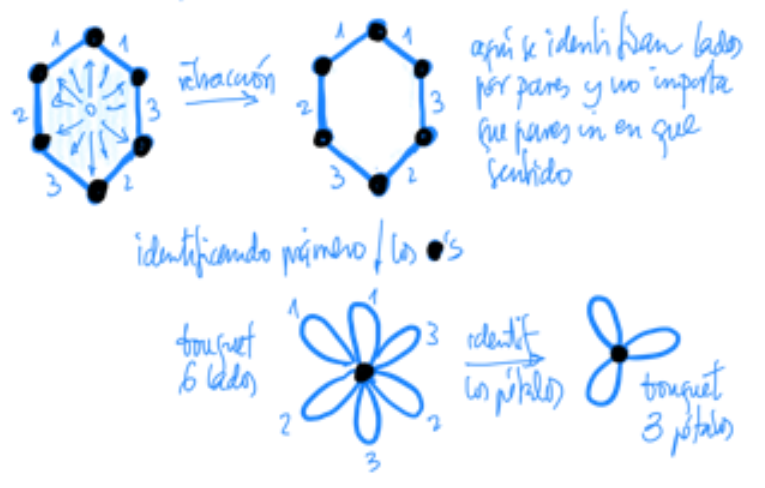
\includegraphics[scale=0.3]{images/dem_grupo_fund_agujeros_3} 
\end{center}
\end{demo}
Con $k$ arbitrario es lo mismo: se empieza con un polígono de $2k$ lados, que se retrae a una poligonal de $2k$ lados, en la que se identifican los vértices para obtener un bouquet de $2k$ pétalos, que se identifican por pares para tener un bouquet de $k$.

\underline{Conclusión}:

Todas las superficies se distinguen por el grupo fundamental después de quitar un punto, salvo los pares:
\[
\Pi^2 \# \stackrel{k}{\cdots} \# \Pi^2\; \land \;\mathbb{P}^{2} \# \stackrel{2k}{\cdots} \# \mathbb{P}^{2} = \mathbb{K}^2 \# \stackrel{k}{\cdots} \# \mathbb{K}^2
\]
para cada $k \ge 1$. El primer caso (y el esencial) es que el toro y la botella de Klein no son homeomorfos: La razón de fondo es la orientabilidad, que no hemos estudiado aquí.

En general:
\begin{itemize}
    \item Cualquier $\mathbb{P}^{n} \# \cdots \# \mathbb{P}^{2}$ contiene una banda de Möbius (de hecho, tantas como sumandos) y la banda es no orientable.
    \item Cualquier $\Pi^2 \# \cdots \# \Pi^2$ es orientable, luego cualquier abierto suyo lo es, luego no puede contener una banda de Möbius.
\end{itemize}


\chapter{Grande finale}%
\label{cha:grande_finale}
Vamos a probar que la esfera \underline{no} es contrátil, utilizando el teorema de la esfera de Brouwer (\ref{sec:teorema_de_la_esfera_de_brouwer}) y las ideas sobre vectores tangentes allí vistas:
\begin{prop}
$\mathbb{S}^{2}$ \underline{no} es contráctil: $\nexists H_t: cte. \simeq id_{\mathbb{S}^{2}}$.
\end{prop}
\begin{demo}
Absurdo: sea que $\exists H_t: \mathbb{S}^{2} \rightarrow \mathbb{S}^{2},\ H_0\left( x \right) = x_0,\ H_1\left( x \right) = x$.
\begin{enumerate}
    \item \underline{Problema de elevación}:
    %TODO: Imagen
    \begin{center}
        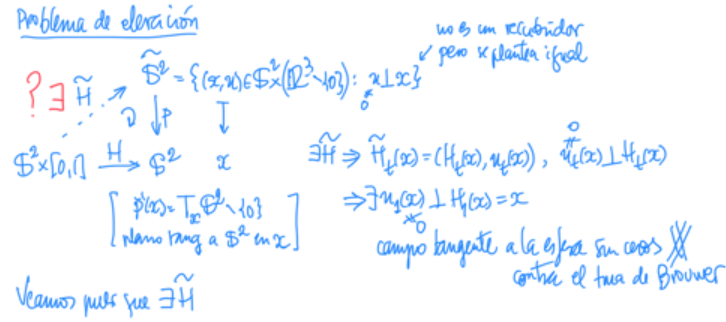
\includegraphics[scale=0.3]{images/prob_elevacion} 
    \end{center}

    %TODO: Fix subrayado
    \item \underline{Estructura de }$\tilde{\mathbb{S}}^1$: 

    Como esquema tenemos,
    %TODO: Imagen
    \begin{center}
        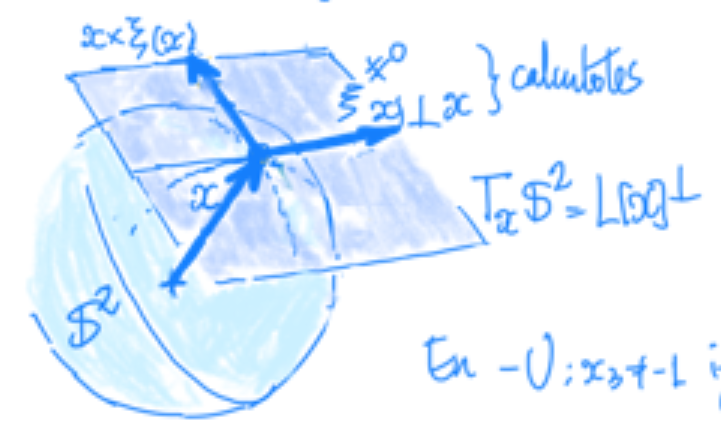
\includegraphics[scale=0.3]{images/esquema_estr_s2} 
    \end{center}
    Así,
        $c = \left( 0, 0, 1 \right),\ U = \mathbb{S}^{2} \setminus \{c\} = \{x_3 \neq 1\},\ -U : \mathbb{S}^{2} \setminus \{-c\} = \{x_3 \neq -1\}$.

    En $U: x_3 \neq 1,\ \{\eta\left( x \right) = \left( 1 - x_3 - x_1^2, -x_1x_2, x_1\left( 1- x_3 \right) \right),\ \eta\left( x \right) = x \times \eta\left( x \right)\}$ base de $T_x\mathbb{S}^{2}$ ortogonal. $\Rightarrow \forall \underbrace{u}_{\neq 0} \perp x: u = \lambda\left( u, x \right) \eta\left( x \right) + \mu\left( u, x \right) \eta\left( x \right)$.
    \[
    \begin{cases}
        \lambda\left( u, x \right) = \langle u, \eta\left( x \right) \rangle / \lVert \eta\left( x \right) \rVert^2\\
        \mu\left( u, x \right) = \langle u, \eta\left( x \right) \rangle / \lVert \eta\left( x \right) \rVert^2
    \end{cases} \text{ cond's ?? continuas.} 
    \]

    En $-U : x_3\neq -1$ igual con $\eta\left( x \right) = \left( 1 + x_3 - x_1^2, -x_1x_2, -x_1\left( 1 + x_3 \right) \right)$.

    \item \underline{Preparación local}: Igual que en $\ref{sec:unicidad_de_elevacion}$ para la elevación de recubridores:
    \begin{align*}
        \forall x \in \mathbb{S}^{2},\ \exists W^x \stackrel{\text{ab.}}{\subset} \mathbb{S}^{2},\ \exists 0 = t_0 < \ldots < t_r = 1 : &W^x \times \left[ t_{i - 1}, t_i \right] \subset H^{-1}\left( U \right) \text{ ó } H^{-1}\left( -U \right)\\
        &\text{reducción } W^x \supset \overline{V^x} \supset V^x
    .\end{align*}
    ¡La partición depende de $x$! $\Rightarrow{\mathbb{S}^{2}\text{ comp.}} \mathbb{S}^{2} = V^{x_1} \cup \ldots \cup V^{x_v}$ y juntamos las $v$ particiones.
    \[
    \Rightarrow \mathbb{S}^{2} = V_1 \cup \ldots \cup V_v\; \land \;\exists 0 = t_0 < \ldots < t_r = 1: H\left( \overbrace{W_k}^{\supset \overline{V}_k \supset V_k} \times \left[ t_{i - 1}, _i \right] \right) \subset U \text{ ó } -U.
    \]

    \underline{Objetivo}: construir la elevación $\tilde{H}$ en pasos sucesivos: 
    \begin{itemize}
        \item dada $\tilde{H}_t$ para $0 \le t \le t_{i-1}$ extenderla a $t_{i - 1} \le t \le t_i$, es decir, 
        \item dada $\tilde{H}_{t_{i - 1}}$ extenderla a $t_{i - 1} \le t \le t_i$.
    \end{itemize}
    Para empezar en $i = 1$: 
    \[
    \tilde{H}_{t_0} \left( x \right) = \tilde{H}_0\left( x \right) = \left( H_0\left( x \right), u_0\left( x \right) \right) = \left( x_0, u_0 \right),\ \text{cualquier } \overbrace{u_0}^{\neq 0} \perp x_0
    \]
    El paso inductivo da más trabajo y para simplificar un escalamiento permite suponer $\left[ t_{i - 1}, t_i \right]\\ = \left[ 0, 1 \right]$ y $H\left( W_k \times \left[ 0, 1 \right] \right) \subset U$ ó $-U\ \forall k$(*). Queremos:
    \begin{itemize}
        \item dada $\tilde{H}_0$ extenderla a $0 \le t \le 1$
        \begin{demo}
            $\tilde{H}_0 = \tilde{H}_{t_i - 1}$ \underline{no} es la elevación de $i = 1$. 
        \end{demo}
    \end{itemize}

    \item \underline{Descomposición de la extensión en varios pasos}: Tomamos $C_k = \mathbb{S}^{2} \setminus V_k$ y,
    \begin{enumerate}
        \item $\varphi_k\left( x \right) = \frac{\mathrm{dist} \left( x, C_k \right)}{\sum_{l} \mathrm{dist} \left( x, C_k \right)} \Rightarrow \begin{cases}
            0 \le \varphi_k \le 1\\
            \{\varphi_k = 0\} = C_k\\
            \sum_{l} \varphi_l = 1 
        \end{cases}$ por ser los $C_k$ cerrados.

        \item $\psi_k = \varphi_1 + \cdots + \varphi_k \Rightarrow \begin{cases}
            0 \equiv \psi_0 \le \psi_1 \le \ldots \le \psi_k \equiv 1\\
            \{\psi_{k - 1} < \psi_k\} = \{\varphi \neq 0\} = X \setminus C_k = V_k (**)\\
            \overline{\{\psi_{k - 1} < \psi_k\}} = \overline{V_k} \subset W_k
        \end{cases}$
    \end{enumerate}
    Las $\psi_k$ son los límites superiores de la siguiente cadena de cerrados:
    \[
    \mathbb{S}^{2} \times \{0\} = \Gamma_0 \subset \Gamma_1 \subset \ldots \subset \Gamma_k = \{t \le \psi_k\left( x \right) : x \in \mathbb{S}^{2}\} \subset  \ldots \subset \Gamma_v = \mathbb{S}^{2} \times \left[ 0, 1 \right] 
    \]
    y, empezando con $\tilde{H}_0$ para $k = 1$, la cosa es:
    \begin{itemize}
        \item dada $\tilde{H}^{k - 1} = \left( r, u^{k - 1} \right)$ elevación de $H|_{\Gamma_{k - 1}}$, extenderla a $\Gamma_k \setminus \Gamma_{k - 1}$. Como:
        \[
        \begin{cases}
            \Gamma_{k - 1} \setminus \overline{V}_k \times \left[ 0, 1 \right] \stackrel{(**)}{=} \Gamma_k \setminus \overline{V}_k \times \left[ 0, 1 \right] = A \stackrel{\text{ab.}}{\subset} \Gamma_k\\
            \Gamma_{k - 1} \cap \left( W_k \times \left[ 0, 1 \right] \right) = B \stackrel{\text{ab.}}{\subset} \Gamma_k
        \end{cases}\land\ \Gamma_k = \underbrace{A}_{\subset \Gamma_{k - 1}} \cup B
        \]
        definiremos,
        \item $\tilde{H}^k$ en $B$ tal que, $\tilde{H}^k = \tilde{H}^{k - 1}$ en $A \cap B \subset \mathbb{S}^{2} \setminus V_k \times \left[ 0, 1 \right]$.
    \end{itemize}

    \item $\left( x, t \right) \in B \xRightarrow{(*)} \begin{cases}
        H_t\left( x \right) \in U\\
        H_{\psi_{k - 1} \left( x \right)} \left( x \right) \in U
    \end{cases} \Rightarrow \exists \eta$ y $S$ en $\begin{cases}
        H_t\left( x \right).\ (ii)\\
        H_{\psi_{k - 1} \left( x \right)} \left( x \right).\ (i)
    \end{cases}$.
    %TODO: Imagen
    \begin{center}
        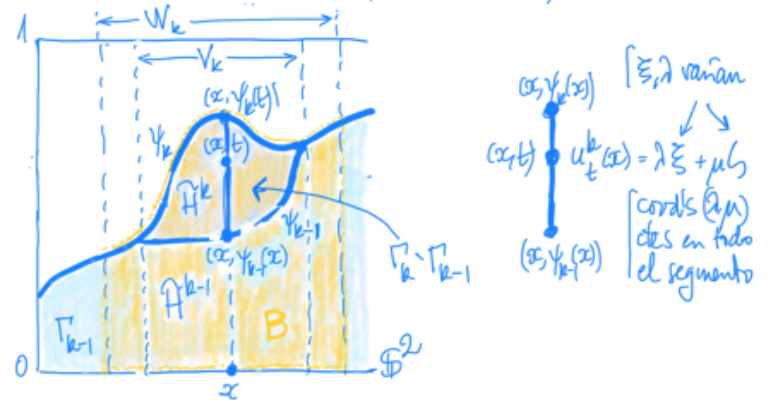
\includegraphics[scale=0.3]{images/finale_5} 
    \end{center}
    \begin{enumerate}
        \item $t \le \psi_{k - 1} \left( x \right) : \left( x, t \right) \in \Gamma_{k - 1} \Rightarrow \tilde{H}_t^k \left( x \right) = \tilde{H}_t^{k - 1} \left( x \right)$.
        \item $t \ge \psi_{k - 1} \left( x \right) : \tilde{H}^{k - 1} = \left( H, u^{k - 1} \right)$.
        \begin{enumerate}
            \item[(i)] $\Rightarrow$
            %TODO: Subíndice sin pareja
            \begin{align*}
            \underbrace{u_{\psi_{k-1} \left( x \right)^{k - 1} \left( x \right)}}_{\neq 0} = \lambda_{\psi_{k - 1} \left( x \right)} \left( x \right) \eta\left( H_{\psi_{k - 1}\left( x \right)} \left( x \right) \right) + _{\psi_{k - 1} \left( x \right)} \left( x \right) \zeta\left( H_{\psi_{k - 1}\left( x \right)} \left( x \right) \right) 
            .\end{align*}
            \item[(ii)] $\Rightarrow$
            \begin{align*}
                \exists u_t^k\left( x \right) &= \lambda_{\psi_{k-1}\left( x \right)} \left( x \right) \eta\left( H_t\left( x \right) \right) + \mu_{\psi_{k - 1} \left( x \right)} \left( x \right) \zeta\left( H_t\left( x \right) \right) \\
                &\Rightarrow \exists \tilde{H}_t^k\left( x \right) = \left( H_t\left( x \right), u_t^k\left( x \right) \right)
            .\end{align*}
            y por la construcción es continua.
        \end{enumerate}

    \item[a) y b)] coinciden en $t = \psi_{k - 1} \left( x \right)$.
    \end{enumerate}

    \item $\psi_{k - 1} \stackrel{(**)}{=} \psi_k$ fuera de $V_k \Rightarrow \tilde{H}^k$ de 5. $= \tilde{H}^{k - 1}$ en $A \cap B$.
\end{enumerate}

Esto completa la propuesta de que $\exists \tilde{H}$ elevación de $H$ y, con ello, se completa la contradicción buscada. Acaba aquí la demostración de que $\mathbb{S}^{2}$ no es contráctil.
\end{demo}

